% !TEX TS-program = pdflatex
% !TEX encoding = UTF-8 Unicode
% This is a simple template for a LaTeX document using the "article" class.
% See "book", "report", "letter" for other types of document.
\documentclass[11pt]{article} % use larger type; default would be 10pt
\usepackage[utf8]{inputenc} % set input encoding (not needed with XeLaTeX)
%%% Examples of Article customizations
% These packages are optional, depending whether you want the features they provide.
% See the LaTeX Companion or other references for full information.
%%% PAGE DIMENSIONS
\usepackage{geometry} % to change the page dimensions
\geometry{a4paper} % or letterpaper (US) or a5paper or....
% \geometry{margin=2in} % for example, change the margins to 2 inches all round
% \geometry{landscape} % set up the page for landscape
% read geometry.pdf for detailed page layout information
\usepackage{graphicx} % support the \includegraphics command and options
% \usepackage[parfill]{parskip} % Activate to begin paragraphs with an empty line rather than an indent
%%% PACKAGES
\usepackage{booktabs} % for much better looking tables
\usepackage{array} % for better arrays (eg matrices) in maths
\usepackage{paralist} % very flexible & customisable lists (eg. enumerate/itemize, etc.)
\usepackage{verbatim} % adds environment for commenting out blocks of text & for better verbatim
\usepackage{subfig} % make it possible to include more than one captioned figure/table in a single float
% These packages are all incorporated in the memoir class to one degree or another...
\usepackage[polish]{babel}	
\usepackage{polski}
\usepackage{mathtools}
\usepackage{amsmath}
\usepackage[pdftex,colorlinks=false,plainpages=false]{hyperref}

\usepackage[T1]{fontenc}
\frenchspacing	
\usepackage{indentfirst}


%%% HEADERS & FOOTERS
\usepackage{fancyhdr} % This should be set AFTER setting up the page geometry
\pagestyle{fancy} % options: empty , plain , fancy
\renewcommand{\headrulewidth}{0pt} % customise the layout...
\lhead{}\chead{}\rhead{}
\lfoot{}\cfoot{\thepage}\rfoot{}
%%% SECTION TITLE APPEARANCE
\usepackage{sectsty}
\allsectionsfont{\sffamily\mdseries\upshape} % (See the fntguide.pdf for font help)
% (This matches ConTeXt defaults)
%%% ToC (table of contents) APPEARANCE
\usepackage[nottoc,notlof,notlot]{tocbibind} % Put the bibliography in the ToC
\usepackage[titles,subfigure]{tocloft} % Alter the style of the Table of Contents
\renewcommand{\cftsecfont}{\rmfamily\mdseries\upshape}
\renewcommand{\cftsecpagefont}{\rmfamily\mdseries\upshape} % No bold!
%%% END Article customizations
%%% The "real" document content comes below...
\title{Sztuczne Sieci Neuronowe \\ \large Sprawozdanie z projektu}
\author{Łukasz Rados, Wojciech Kusa \\ Wydział Fizyki i Informatyki Stosowanej \\ Akademia Górniczo-Hutnicza im. Stanisława Staszica w Krakowie}

%\date{} % Activate to display a given date or no date (if empty),
% otherwise the current date is printed


\begin{document}
\maketitle

\section{Wprowadzenie}
Celem opisywanego projektu było zaimplementowanie i próba nauczenia sieci neuronowej grania w prostą grę komputerową. Genezą projektu jest publikacja [1], w której autorzy próbują nauczyć sieć neuronową za pomocą metody tzw. \textit{deep learning} algorytmów grania w różne gry komputerowe wydane na platformę Atari. Naszą motywacją było stworzenie gry komputerowej wzorującej się na grze \textit{T-Rex Runner} znajdującej się w przeglądarce Google Chrome [2], a następnie zaimplementowanie takiej struktury sieci neuronowej, która byłaby w stanie nauczyć się skutecznie grać w tę grę. \\

Rozważane zostały różne rodzaje reprezentacji planszy gry (opisujące różne poziomy abstrakcji) oraz wpływ technik uczenia sieci na jakość działania. Ze względu na ograniczenia implementacyjne przetestowane zostało działanie tylko sieci o strukturze radialnej. Uzyskane wyniki (pomimo iż opracowane przypadki były relatywnie proste) są zadowalające oraz stanowią podstawę i dobry punkt wyjścia do dalszego rozwoju projektu. \\

Projekt został wykonany w języku Python 2.7/3.4 z wykorzystaniem bibliotek do obliczeń numerycznych NumPy, SciPy oraz biblioteki wspomagającej proces tworzenia gier komputerowych PyGame.\\


\section{Podstawy teoretyczne}

Problem przyswajania przez algorytmy uczenia maszynowego algorytmów dotyczących innych dziedzin (zadań) jest najczęściej sprowadzany do problemu klasyfikacji i rozpoznawania wzorca. Podstawowymi elementami, które są różne dla tych zadań jest sposób reprezentacji przestrzeni stanu (problemu) oraz sprzężenie zwrotne sygnalizujące jakość odpowiedzi układu. \\

\subsection{Gra}

W ramach tego projektu zaimplementowana została gra komputerowa bazująca na grze \textit{T-Rex Runner}. \textit{T-Rex Runner} jest jednowymiarową grą operująca na niewielkiej przestrzeni możliwych stanów (kilka rodzajów kaktusów oraz latający pterodaktyl) oraz dwóch możliwych ruchach (skok i przykucnięcie). Dzięki tym właściwościom i nieskomplikowanemu interfejsowi człowiekowi bardzo prosto jest opisać jej reguły a skuteczność grania sprowadza się tylko do refleksu. \\

Gra została zaimplementowana z wykorzystaniem biblioteki PyGame do tworzenia gier komputerowych [3]. Zrzut ekranu przedstawiający działającą grę znajduje się na Rysunku \ref{fig:dinosaur_1}.Wychodząc od najprostszej wersji gry czyli z dyskretnym przesunięciem oraz trzema rodzajami obiektów do testów działania sieci neuronowej przygotowano kilka dodatkowych rozszerzeń utrudniających rozgrywkę takich jak ciągły skok dinozaura czy dodatkowy typ kaktusa. \\


\begin{figure}[h]
\centering
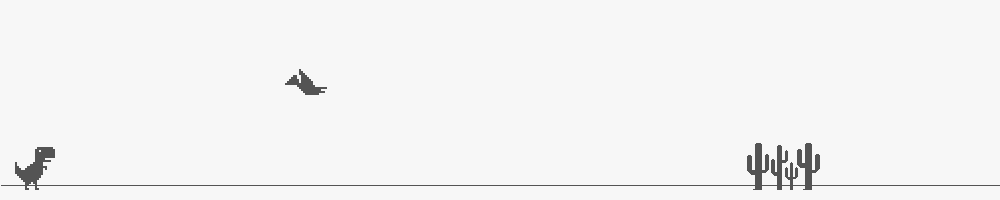
\includegraphics[width=10cm]{images/dinosaur_1}
\caption{Zrzut ekranu przedstawiający grę.} \label{fig:dinosaur_1}
\end{figure}


%\begin{figure}[h]
%\centering
%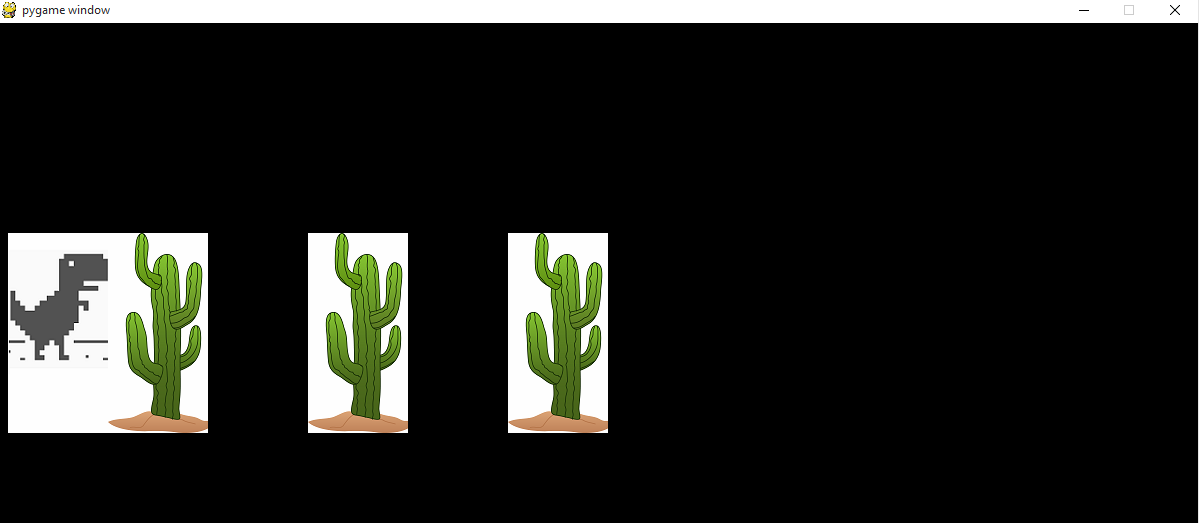
\includegraphics[width=10cm]{images/dinosaur_2}
%\caption{Stan planszy, w którym nie ma działania pozwalającego na przeżycie dinozaura.} \label{fig:dinosaur_2}
%\end{figure}


\subsection{Reprezentacja problemu}

W wersji podstawowej gry plansza opisana jest w postaci macierzy liczb całkowitych o rozmiarze $10 \times 2$ będącej reprezentacją obiektów znajdujących się na planszy. Przykładowo, plansza przedstawiona na Rysunku \ref{fig:dinosaur_1} opisana będzie przez macierz:

\begin{center}

$\begin{bmatrix} 
  0 & 0 & 0 &  3 & 0 & 0 & 0 & 0 & 0 & 0 \\
  1 & 0 & 0 &  0 & 0 & 0 & 0 & 0 & 2 & 0 
 \end{bmatrix}$
\end{center}

Reprezentacja ta, wydaje się prosta ale generuje problemy przy próbie uczenia takiej sieci z powodu dużej liczby połączeń w warstwie ukrytej. Natomiast nauczona sieć dawała bardzo dobre rezultaty, nawet gdy do położenia obiektów wprowadzono rozmyte wartości (prawdopodobieństwo wystąpienia obiektu w tym miejscu). \\

Rozważania była też niskopoziomowa odmiana powyższej metody gdzie plansza byłą reprezentowana przez piksele, a nie obiekty. Jednak opisanie planszy za pomocą pikseli (nawet binarnie) okazało się zadaniem znacznie wykraczającym poza możliwości normalnych komputerów, gdyż trenowanie takiej sieci zajmowało zdecydowanie za dużo czasu a sieć pomimo swoich ogromnych rozmiarów (nawet przy niewielkiej rozdzielczości ekranu było to co najmjiej $10^7$ połączeń) nie dawała sobie rady z rozwiązaniem problemu. Podstawową kwestią jest tutaj konieczność dokonywania meta-klasyfikacji (piksele trzeba najpierw pogrupować w obiekty i dopiero wtedy można dokonywać klasyfikacji ruchów dinozaura) przez sieć do czego potrzebna jest inna struktura i inny sposób uczenia sieci. \\

Z powyższych względów zdecydowano się też na przetestowanie innego sposobu reprezentacji planszy gry. Plansza opisana została przez $n$ pierwszych elementów znajdujących się na niej. Pominięte zostały wszystkie puste pola co znacznie zmniejszyło liczbę danych wejściowych ale jednocześnie nie uprościło znacząco rozgrywki gdyż w dalszym ciągu gracz musi zadecydować czy ta względna odległość jest wystarczająca aby wykonać skok i ominąć przeszkodę. \\

Na początku opracowana została reprezentacja, w której każdy obiekt opisany jest przez 3 wielkości ($x_1$ - początkowe położenie poziome, $x_2$ - końcowe położenie poziome oraz $y$ - typ obiektu, Rysunek \ref{fig:representation}). Tak stworzoną reprezentację z łatwością można rozbudowywać o dodatkowe parametry ''utrudniające'' rozgrywkę takie jak: 

\begin{itemize}
\item liczbę analizowanych obiektów,

\item rozmycie położenia obiektów,

\item wprowadzenie rozmiaru obiektu w osi $y$ zamiast jego typu.

\end{itemize} 

\begin{figure}[h]
\centering
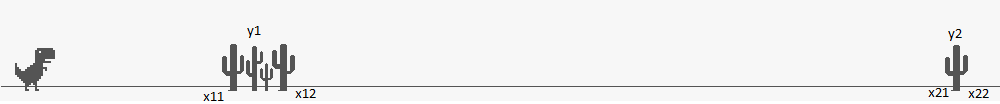
\includegraphics[width=12cm]{images/representation}
\caption{Drugi sposób reprezentacji planszy gry.} \label{fig:representation}
\end{figure}


\subsection{Sieć Neuronowa}
 
Sieć radialna (ang. \textit{radial basis function network, RBFN}) jest odmianą sigmoidalnej iteracyjnej sieci neuronowej. Neuron takiej sieci reprezentuje hipersferę dokonując posziału kołowego. Jego funkcją aktywacji jest funkcja radialna, na przykład $\phi (r) = e^{-\frac{r^2}{\beta}}$ . Model sieci radialnej przedstawiony został na Rysunku \ref{fig:radial_network}. \\


\begin{figure}[h]
\centering
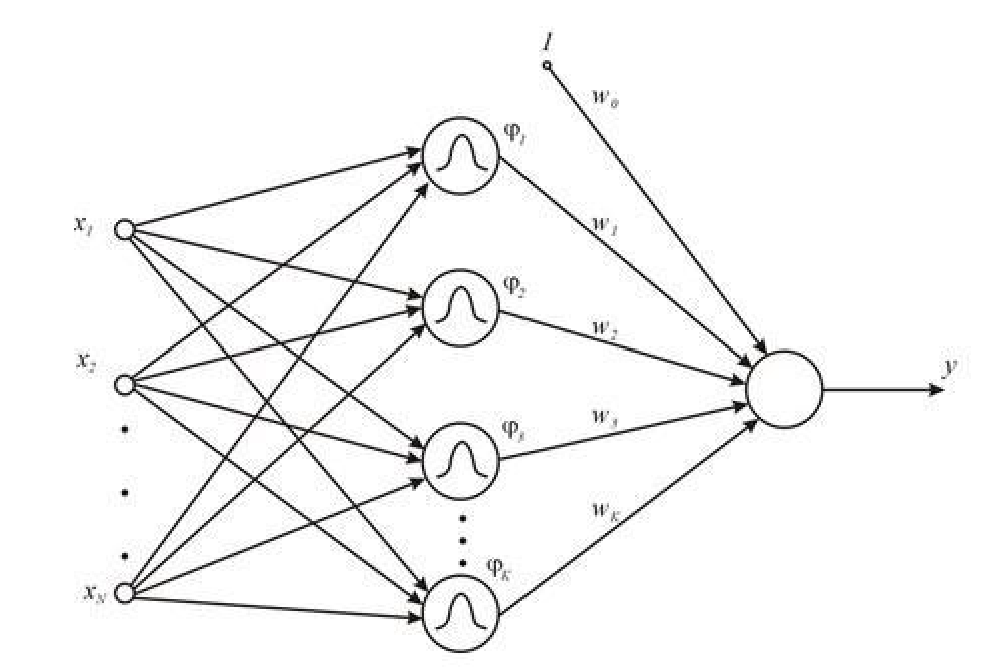
\includegraphics[width=12cm]{images/radial_network}
\caption{Model sieci radialnej.} \label{fig:radial_network}
\end{figure}

Proste sieci radialne działają na zasadzie interpolacji wielowymiarowej, w której $n$ różnych wektorów wejściowych jest odwzorowywanych z przestrzeni $N$-wymiarowej w zbiór k liczb rzeczywistych $d_i, {i = 1, 2, ..., k}$. \\


Sieci radialne z powodzeniem stosowane były w rozwiązywaniu problemów klasyfikacyjnych, zadaniach aproksymacyjnych oraz zagadnieniach predykcji czyli wydają się idealnym narzędziem do nauki algorytmu gry w opisanych wyżej sposobach reprezentacji przestrzeni stanów. \\

W projekcie wykorzystano implementację sieci radialnej pyradbas [4] dostosowując ją do specyfiki problemu (generowanie odpowiedzi na bieżąco w trakcie gry). \\

\section{Wyniki}

Ze względu iż trenowanie sieci podczas reprezentacji obejmującej macierz obiektów znajdujących się na planszy zajmowało bardzo dużo czasu sposób ten został uznany za nieefektowny przy wybranej strukturze sieci i pominięto go podczas dalszych eksperymentów. \\

%\includemovie{5cm}{5cm}{gif/jumping.gif}

Przestestowane zostało zatem działanie sieci neuronowej dla reprezentacji względnego położenia obiektów na planszy. Sieć trenowana jest za pomocą obserwacji ruchów gracza czlowieka przy konkretnym stanie planszy podczas kilku uruchomień gry, a następnie testowana jest gdy podczas uruchomionej gry musi ''w locie'' przewidywać następny ruch. \\


Średnie wartości punktów uzyskane przez sieć w zależności od liczby analizowanych obiektów przedstawione zostały w Tablicy \ref{tab:results}. Gdy sieć bierze pod uwagę tylko jeden obiekt (na wejściu otrzymuje 3 parametry) to potrafi bezbłędnie przewidzieć następny ruch. Przy zwiększaniu liczby parametrów jej sprawność pogarasza się znacząco - przy 4 obiektach nie potrafi wykonać nawet jednego skoku. Wyniki te nie są uzależnione od rozmiaru zbioru treningowego - dla 50 elementów treningowych sieć uzyskuje takie same wyniki jak na dla zbioru treningowego zawierającego 2000 przypadków. \\


\begin{table}[]
\centering
\caption{Wyniki uzyskane przez sieć neuronową.}
\label{tab:results}
\begin{tabular}{|l|l|l|}
\hline
{\bf Liczba analizowanych obiektów} & {\bf Średni wynik sieci} & {\bf Odchylenie standardowe} \\ \hline
1                                   & inf                      & 0                            \\ \hline
2                                   & 635.2                    & 21.1                         \\ \hline
3                                   & 105.8                    & 16.4                         \\ \hline
4                                   & 72.5                     & 3.3                          \\ \hline
\end{tabular}
\end{table}

Wartości pobrane z planszy były dodatkowo zaburzane niewielkimi wartościami szumem gaussowskim


Sprawdzone zostało też, jak zmienia się wartość wyniku uzyskanego przez sieć neuronową w zależności od rozmycia położenia obiektów na planszy (przyjęto że 1- całkowite rozmycie, 0 - brak rozmycia). Wyniki symulacji znajdują się na Rysunku \ref{fig:fuzzyfication_score}. Gdy rozmycie nie występuje sieć potrafi grać w nieskończoność, co można zaobserwować na wykładniczym wzroście liczby zdobytych punktów przez sieć. Ciekawy jest też fakt, że dla rozmycia z zakresu $[0.1, 1]$ praktycznie nie zmienia się średnia liczba zdobytych punktów. Świadczyć to może o tym, że ten typ sieci dosyć słabo radzi sobie z parametrami podanymi w sposób rozmyty. \\


\begin{figure}[h]
\centering
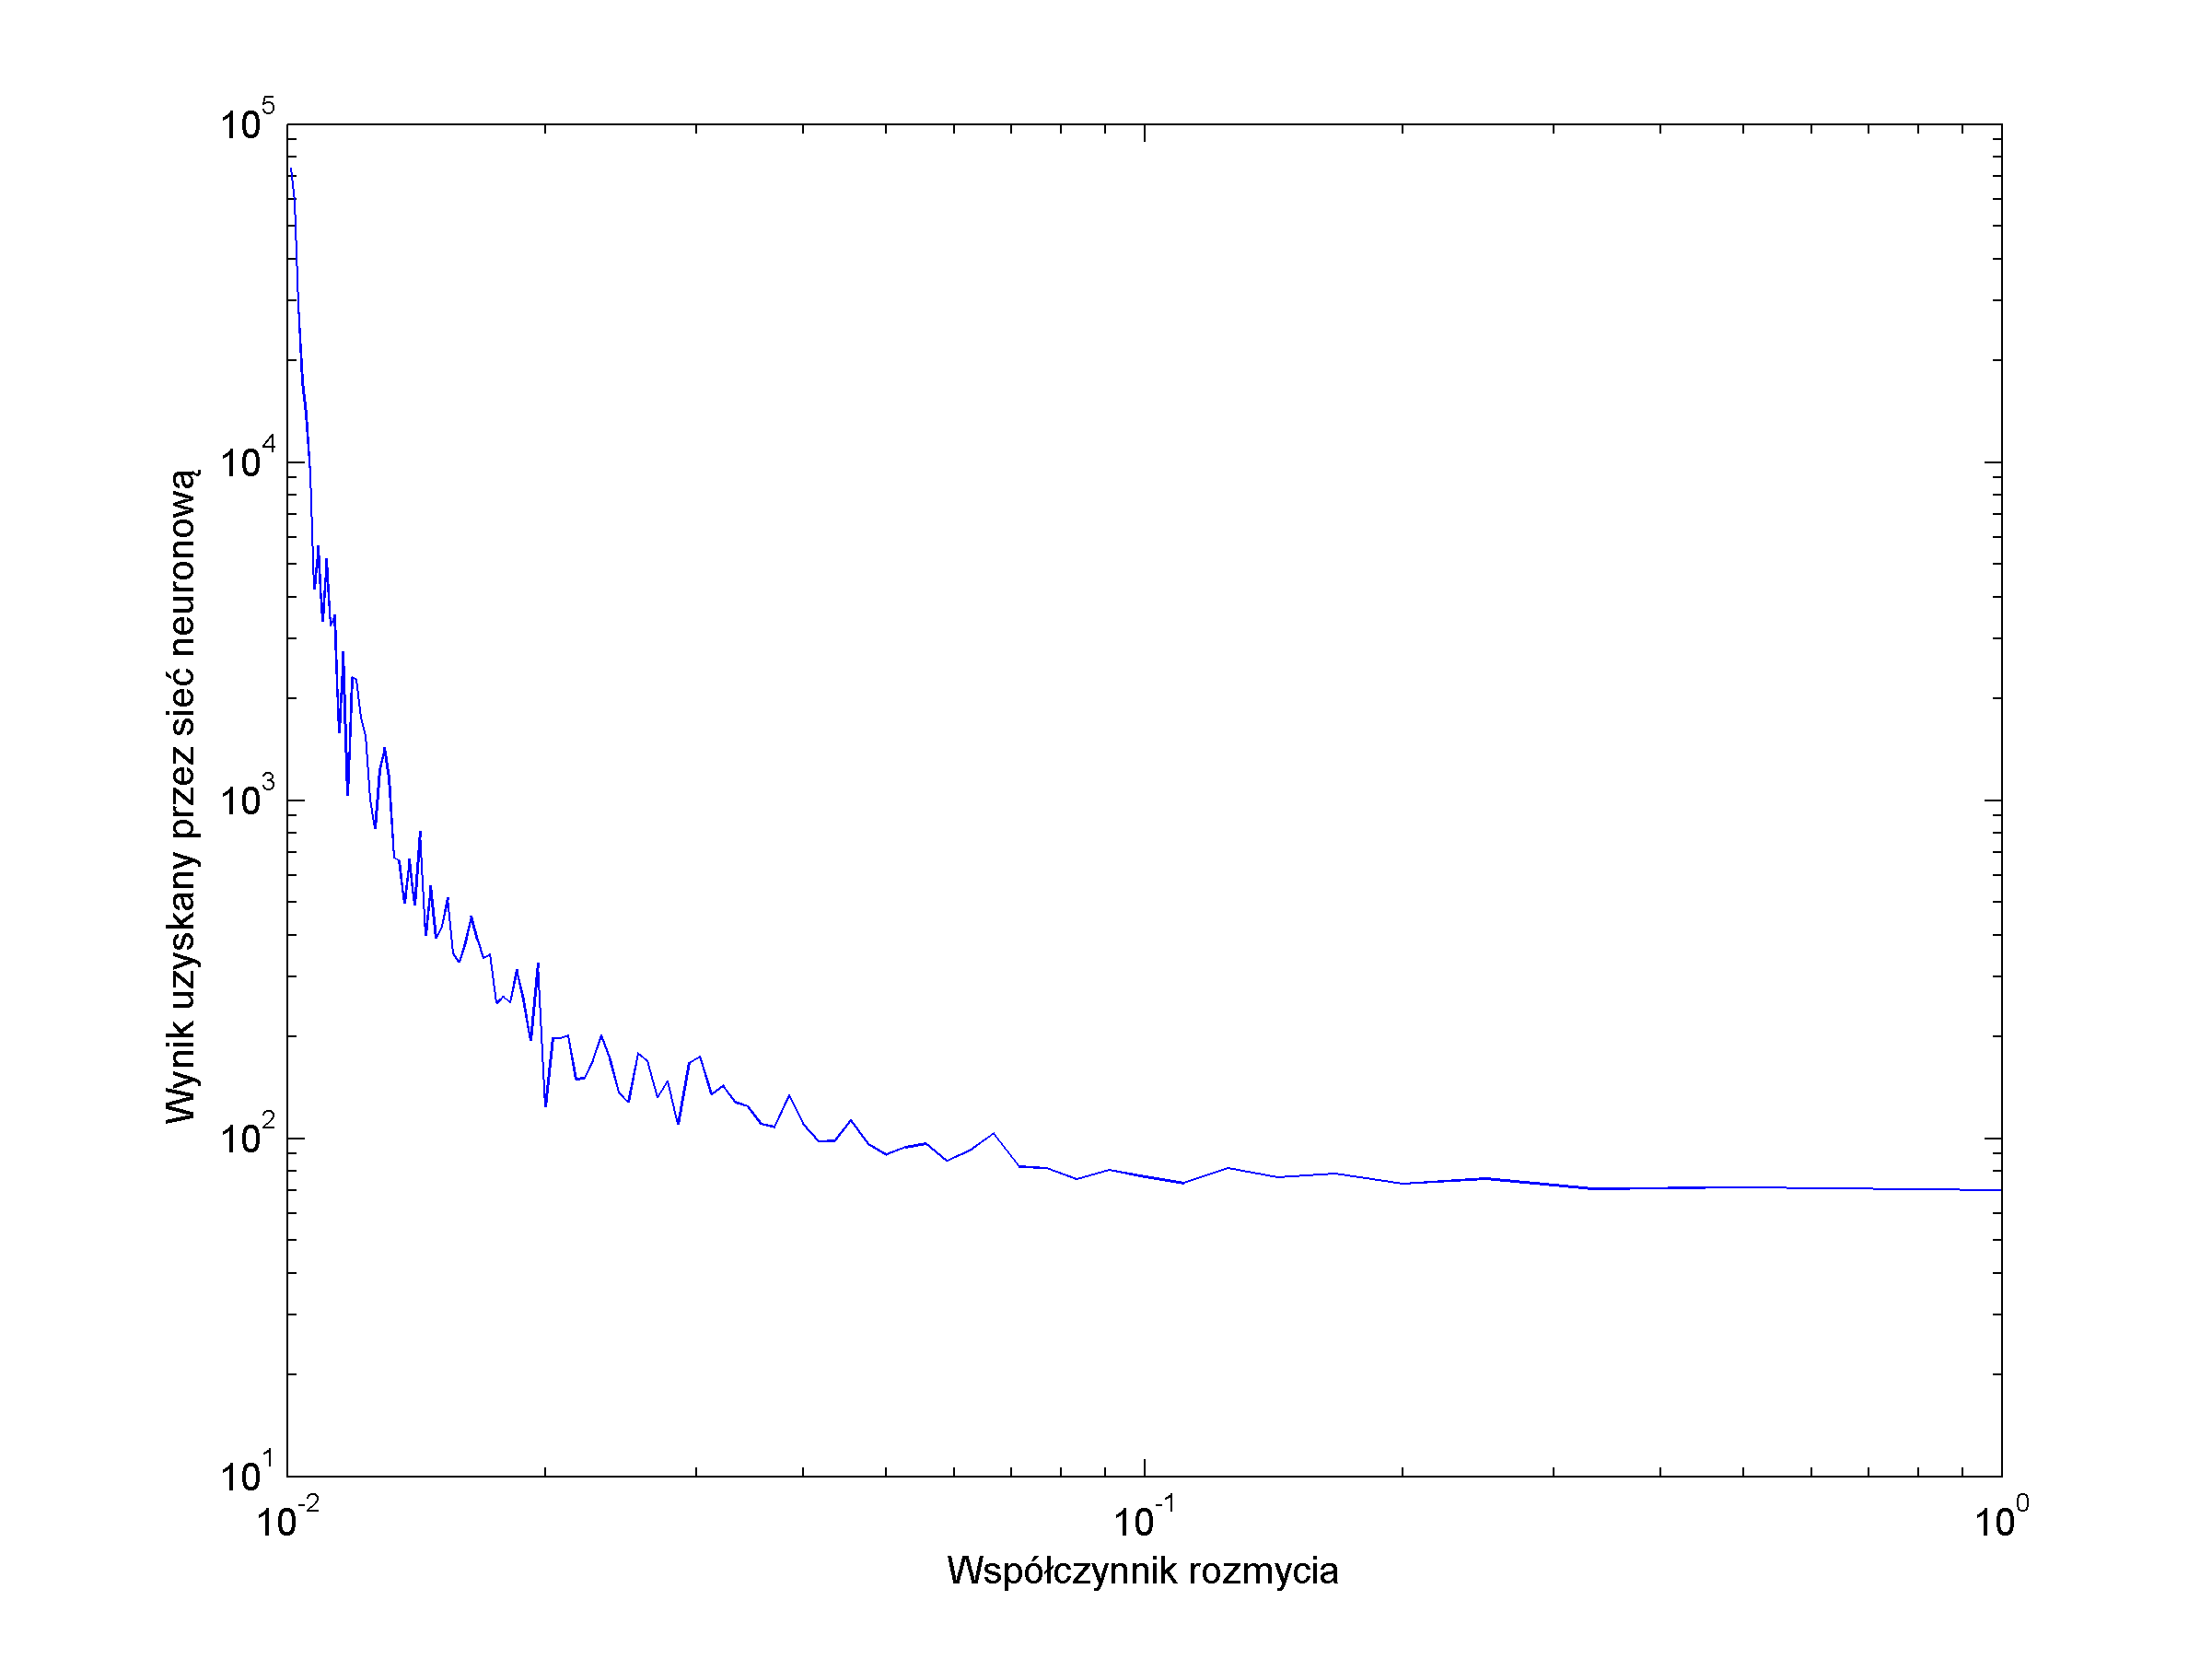
\includegraphics[width=12cm]{images/fuzzyfication_score}
\caption{Liczba uzyskanych punktów przez sieć neuronową w zależności od współczynnika rozmycia danych (1- całkowite rozmycie, 0 - brak rozmycia). Skala wykresu loglog.} \label{fig:fuzzyfication_score}
\end{figure}





\section{Podsumowanie}

Uzyskane wyniki świadczą, że przy odpowiednio przygotowanej reprezentacji planszy jest możliwość nauczenia sieci neuronowej o strukturze radialnej reguł grania w proste jednowymiarowe gry komputerowe. Oczywiście dzieje się tak ponieważ rozwiązywany problem posiada prosty opis i jest możliwy podział (klasyfikacja) zbioru odpowiedzi na grupy. \\

Z powodów ograniczonych zasobów komputerowych nie było możliwe zreplikowanie eksperymentów zaprezentowanych w [1], gdyż próba nauczenia sieci neuronowej za pomocą standardowych metod zajęłaby nierealistycznie dużo czasu a zmniejszenie ilości neuronów w sieci powodowało kompletne nieradzenie sobie jej z tym zadaniem. Z powyższych względów postanowiono ograniczyć przestrzeń problemu i spróbować rozwiązać go rozwiązać na wyższym poziomie abstrakcji. Ciekawym rozwiązaniem mogłoby być jedna

\section*{Bibliografia}
\begin{enumerate}
\item V Mnih, K Kavukcuoglu, D Silver, A Graves, I Antonoglou, D Wierstra, M Riedmiller - Playing Atari with Deep Reinforcement Learning. NIPS 2013 Deep Learning Workshop

\item http://www.omgchrome.com/chrome-easter-egg-trex-game-offline/

\item http://www.pygame.org/hifi.html

\item https://github.com/cybercase/pyradbas

\end{enumerate}

\section*{Załączniki}

\begin{itemize}

\item game.wmv - animacja prezentująca efekt działania sieci neuronowej w trakcie gry

\end{itemize}

\end{document}

